\clearpage

\section{White Noise}

\begin{tcolorbox}	
	\begin{tabular}{p{2.75cm} p{0.2cm} p{10.5cm}} 	
		\textbf{Header File}   &:& white\_noise\_20180118.h \\
		\textbf{Source File}   &:& white\_noise\_20180118.cpp \\
	\end{tabular}
\end{tcolorbox}

\maketitle
This block generates a gaussian pseudo-random noise signal with a given spectral density. It can be initialized with three different seeding methods:

%\begin{multicols}{2}
\begin{enumerate}
	\item DefaultDeterministic
	\item RandomDevice
	\item Selected
\end{enumerate}
%\end{multicols}

This block does not accept any input signal. It produces can produce a real or complex output, depending on the used output signal. If the signal is complex, the noise is calculated independently for the real and imaginary parts, with half the spectral density in each.

\subsection*{Input Parameters}

%	\begin{itemize}
%		\item mode\{PseudoRandom\}\linebreak
%		(Random, PseudoRandom, DeterministicCyclic, DeterministicAppendZeros)
%		\item probabilityOfZero\{0.5\}\linebreak
%		(real $\in$ [0,1])
%		\item patternLength\{7\} \linebreak
%		(integer $\in$ [1,32])
%		\item bitStream\{"0100011101010101"\} \linebreak
%		(string of 0's and 1's)
%		\item numberOfBits\{-1\} \linebreak
%		(long int)
%		\item bitPeriod\{1.0/100e9\} \linebreak
%		(double)
%	\end{itemize}

\begin{table}[h]
	\centering
	\begin{tabular}{|c|c|c|c|c}
		\cline{1-4}
		\textbf{Parameter} & \textbf{Type} &\textbf{Values} &   \textbf{Default}& \\ \cline{1-4}
		seedType 		 & enum & DefaultDeterministic, RandomDevice, Selected & RandomDevice \\ \cline{1-4}
		spectralDensity  & real & > 0  			& $10^{-4}$ \\ \cline{1-4}
		seed 	   		 & int & $\in$ [1, $2^{32}-1$] 	& 1 \\ \cline{1-4} \cline{1-4}
	\end{tabular}
	\caption{White noise input parameters}
	\label{table:bin_sour_in_par}
\end{table}

\subsection*{Methods}

WhiteNoise(vector<Signal *> \&InputSig, vector<Signal *> \&OutputSig) :Block(InputSig, OutputSig){};
\bigbreak	
void initialize(void);
bool runBlock(void);
\bigbreak
void setNoiseSpectralDensity(double SpectralDensity) { spectralDensity = SpectralDensity; }
double const getNoiseSpectralDensity(void){ return spectralDensity; }
\bigbreak
void setSeedType(SeedType sType){ seedType = sType; };
SeedType const getSeedType(void){ return seedType; };
\bigbreak
void setSeed(int newSeed) { seed = newSeed; }
int getSeed(void){ return seed; }

\subsection*{Functional description}

The \textit{seedType} parameter allows the user to select between one of the three seeding methods to initialize the pseudo-random number generators (PRNGs) responsible for generating the noise signal.

\subparagraph*{DefaultDeterministic}
Uses default seeds to initialize the PRNGs. These are different for all generators used within the same block, but remain the same for sequential runs or different \textit{white\_noise} blocks. Therefore, if more than one \textit{white\_noise} block is used, another seeding method should be chosen to avoid producing the exact same noise signal in all sources.

\subparagraph*{RandomDevice}
Uses randomly chosen seeds using \textit{std::random\_device} to initialize the PRNGs.

\subparagraph*{SingleSelected}
Uses one user selected seed to initialize the PRNGs. The selected seed is passed through the variable \textit{seed}. If more than one generator is used, additional seeds are created by choosing the next sequential integers.

%\subparagraph*{AllSelected}
%Uses user selected seeds to initialize the PRNGs. The selected seed is passed through the variable \textit{seed}. If more than one generator is used, additional seeds are created by choosing the next sequential integers.

\subparagraph*{DeterministicCyclic Mode}
Generates the sequence of 0's and 1's specified by \textit{bitStream} and then repeats it.

\subparagraph*{DeterministicAppendZeros Mode}
Generates the sequence of 0's and 1's specified by \textit{bitStream} and then it fills the rest of the buffer space with zeros.

\subsection*{Input Signals}


\subparagraph*{Number:} 0

\subparagraph*{Type:} Binary (DiscreteTimeDiscreteAmplitude)

\subsection*{Output Signals}

\subparagraph*{Number:} 1 or more

\subparagraph*{Type:} Binary (DiscreteTimeDiscreteAmplitude)

\subsection*{Examples}

\paragraph*{Random Mode}

\paragraph*{PseudoRandom Mode}
As an example consider a pseudorandom sequence with \textit{patternLength}=3 which contains a total of 7 ($2^3-1$) bits. In this sequence it is possible to find every combination of 0's and 1's that compose a 3 bit long subsequence with the exception of $000$. For this example the possible subsequences are $010$, $110$, $101$, $100$, $111$, $001$ and $100$ (they appear in figure \ref{BinarySequenceN3} numbered in this order). Some of these require wrap.

\begin{figure}[h]
	\centering
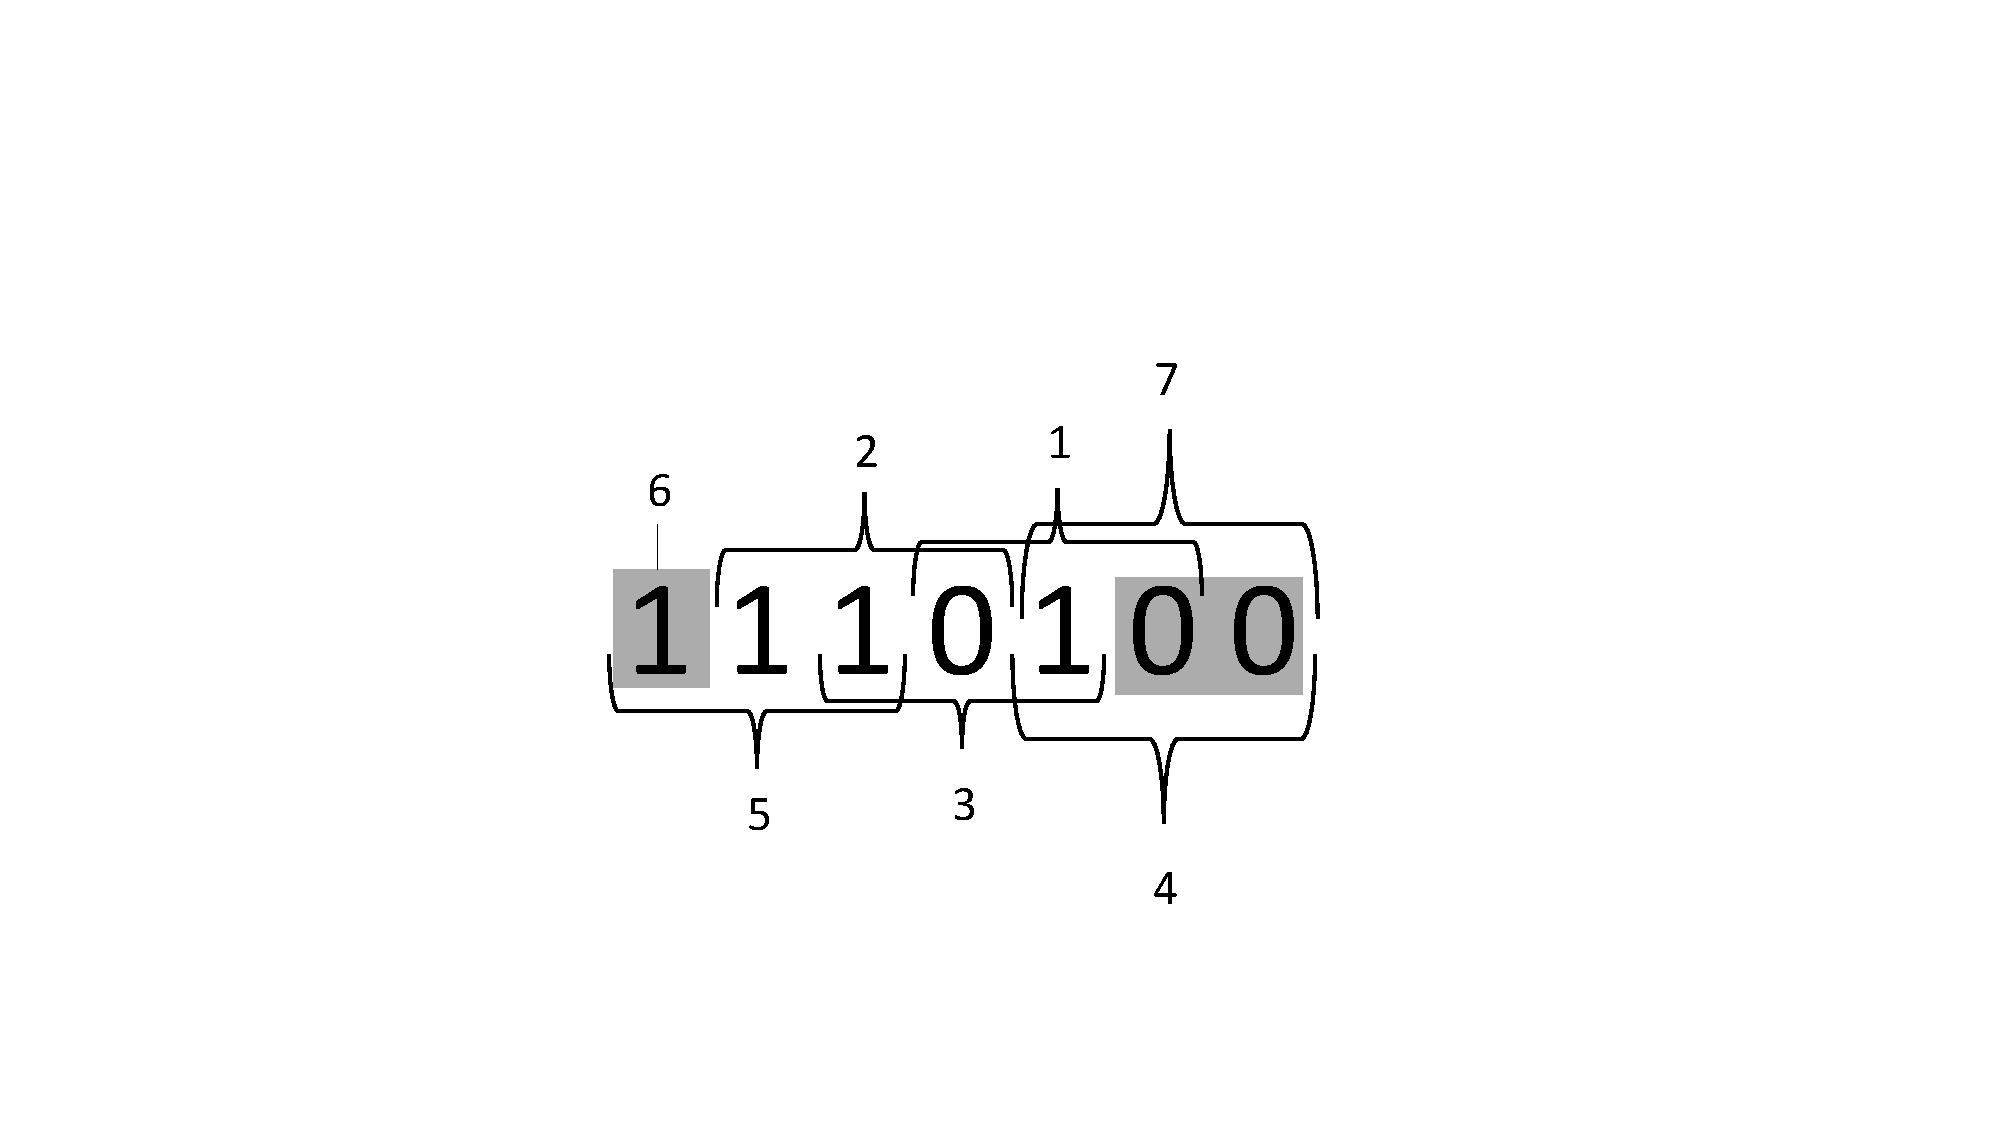
\includegraphics[width=\textwidth]{./lib/binary_source/figures/BinarySequenceN3.pdf}
\caption{Example of a pseudorandom sequence with a pattern length equal to 3.}\label{BinarySequenceN3}
\end{figure}

\paragraph*{DeterministicCyclic Mode}

As an example take the \textit{bit stream} '0100011101010101'. The generated binary signal is displayed in.

\paragraph*{DeterministicAppendZeros Mode}

Take as an example the \textit{bit stream} '0100011101010101'. The generated binary signal is displayed in \ref{MQAM1_DeterministAppendZeros}.

\begin{figure}
	\centering
	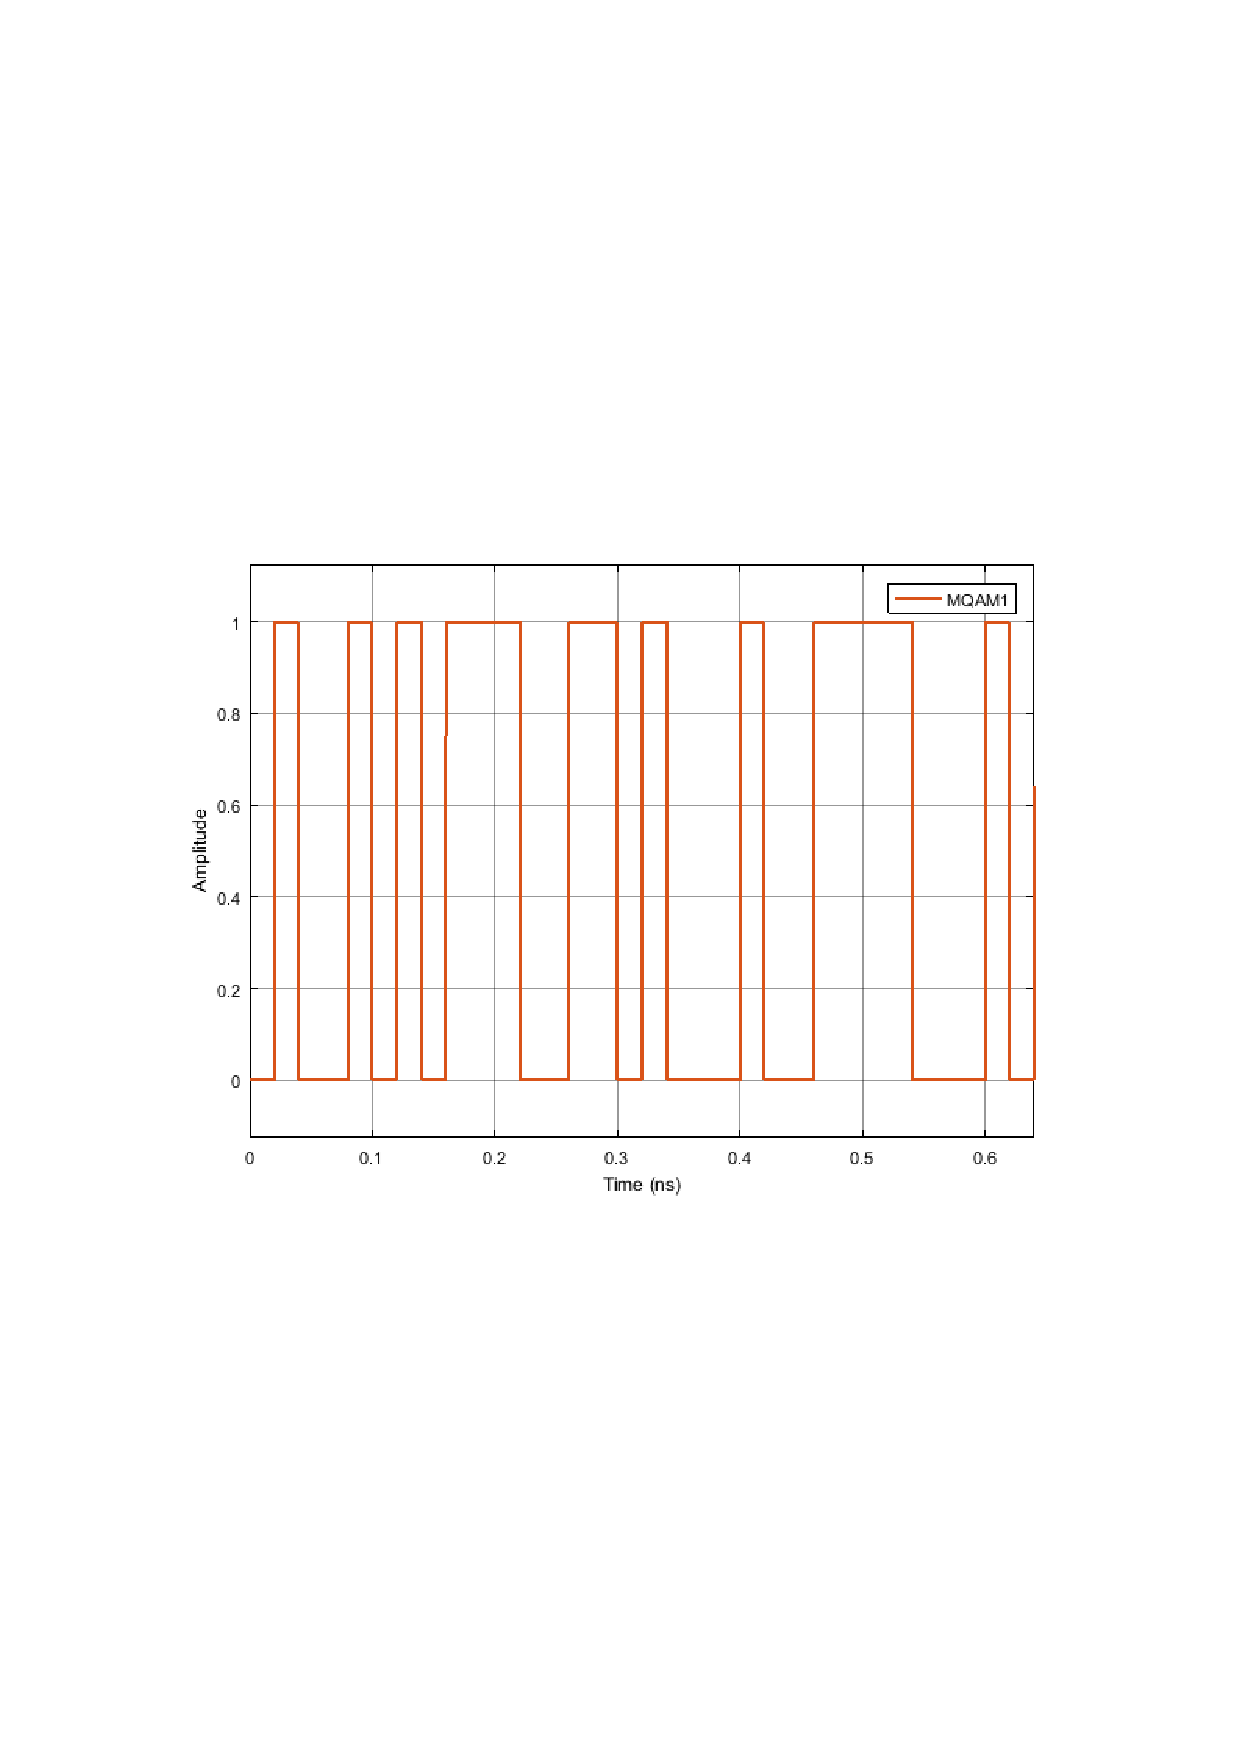
\includegraphics[clip, trim=0.5cm 9cm 0.5cm 9cm, width=\textwidth]{./lib/binary_source/figures/BinarySource_output.pdf}
	
	\caption{Binary signal generated by the block operating in the \textit{Deterministic Append Zeros} mode with a binary sequence 01000...}\label{MQAM1_DeterministAppendZeros}
\end{figure}

\subsection*{Suggestions for future improvement}

Implement an input signal that can work as trigger.

